\chapter{Code versions}
\label{chap:code_versions}

\section{init\_SFU\_state}
\label{sec:init_SFU_state}

\subsection{init\_SFU\_state\_1}
\label{sec:init_SFU_state_1}
  
\begin{verbatim}
!! data_ecc.f95
! sfu_state(1..NSFU) :: normal CRU
  SUBROUTINE init_SFU_state(N_L, mL, Mbig, U_Ro, irow_R, sfu_state)
\end{verbatim}

\subsection{init\_SFU\_state\_2}
\label{sec:init_SFU_state_2}

When peripheral RyRs are incorporated in the model 

\begin{verbatim}
!! data_ecc.f95
! sfu_state(1..NSFU) :: normal CRU
! sfu_state(NSFU+1..) :: peripheral RyR
  SUBROUTINE init_SFU_state_2(N_L, mL, Mbig, U_Ro, irow_R, sfu_state)
\end{verbatim}

\section{get\_compPdt (find rate transition)}
\label{sec:get_compPdt}

Find the current transition rate that a CRU will remain in its current
state. The maximum current transition rate of all CRUs will be used to determine
the next time step. 

\subsection{getCompPdt\_2state}
	
Being used in Leak model that work with 2-state RyR only. 
\begin{verbatim}
CALL getCompPdt_2state<<<gridSize, blocksize>>>()
cuErr = cudaThreadSynchronize()
\end{verbatim}
Here, \verb!compPdt! is an array with fixed 3 columns. 

\subsection{get\_compPdt\_1}
\label{sec:get_compPdt_1}

This version is being used in the Leak model

\begin{verbatim}
CALL getCompPdt_1<<<gridSize, blocksize>>> (kva, kvi)
\end{verbatim}

Here, even though we use only the first column, all other columns are being
computed. As a result, to avoid unncessary calculation, we advance to the next
verion which is set by the macro (Sect.\ref{sec:get_compPdt_2})
\begin{verbatim}
 _USE_NEW_METHOD_ == 1
\end{verbatim}

\subsection{get\_compPdt\_2}
\label{sec:get_compPdt_2}

This version is being used in ECC coupling model.

In this version, we have two copies: one to deal with normal CRUs, and one for
testing with orphan CRUs. Here, the orphan CRUs is modeled in which the coupling
between RyR in a cluster is decreased. 
\begin{verbatim}
#if _TEST_NEW_ORPHAN_CRU_ == _YES 
   CALL get_compPdt_2b <<<gridSize, blocksize>>> (kva, kvi, NSFU_normal, Ej_orphan)
#else
   CALL get_compPdt_2 <<<gridSize, blocksize>>> (kva, kvi)   
#endif
\end{verbatim}


\subsection{get\_compPdt\_3}
\label{sec:get_compPdt_3}

This version is being used in the spatial model. 

In this version, it supports using transformed or non-trasnformed form of
compact-form matrices. Also, it support caffeine testing condition where
opening rate is increased by a factor of, say 1000x. Similarly, we also have 2
versions (one to deal with orphan CRUs)
\begin{verbatim}
#if _TEST_NEW_ORPHAN_CRU_ == _YES 
   CALL get_compPdt_3b <<<gridSize, blocksize>>> (kva, kvi, NSFU_normal, $
    Ej_orphan, time) 
#else
   CALL get_compPdt_3 <<<gridSize, blocksize>>> (kva, kvi, time)   
#endif
   cuErr = cudaDeviceSynchronize()
\end{verbatim}

In Atrial cell, the modified version accepts an additional parameter
\begin{verbatim}
CALL get_compPdt_3 <<<gridSize, blocksize, 0, stream0 >>> (kva, kvi, time,
          Ca_myo_1_dev(PADDING_D+1:)) 
\end{verbatim}

\subsection{get\_compPdt\_Sun2000}
\label{sec:get_compPdt_Sun2000}

\verb!get_compPdt_Sun2000()! function is used to work with LCC Sun2000 model,
and use the new algorithm (MVMC version 2). Here, we also use the new dynamics
buffer in the subspace. There are two versions: one to work with the ventricular
model, and one to work with the atrial cell model.

Ventricular model:
\begin{verbatim}
  CALL get_compPdt_Sun2000 <<<gridSize, blocksize>>> (time) 
\end{verbatim}

Atrial model: the \verb!Ca_myo_1_dev! need to be passed as there is no subspace
and the RyR channels sense the local myoplasmic calcium. Currently, there is no
LCC model is added here
\begin{verbatim}
 CALL get_compPdt_Sun2000_v2 <<<gridSize, blocksize>>> (time,
                 Ca_myo_1_dev(PADDING_D+1:))  
\end{verbatim}


\subsection{get\_compPdt\_rogue}
\label{sec:get_compPdt_rogue}

The gating of rogueRYR has lumenal calcium dependent use the calcium form the
nearby NSR gridpoint.

\begin{verbatim}
CALL get_compPdt_rogue <<< gridSize_rogueRYR, blocksize, 0, stream1>>> (kva, kvi, time, 
       Ca_myo_1_dev(PADDING_D+1:), &                                                                                                
       Ca_nsr_1_dev(PADDING_D+1:), num_rogueRYRcluster, Ej_rogue, N_R_rogue)
\end{verbatim}

\subsection{get\_compPdt\_rogue\_3 (atrial)}
\label{sec:get_compPdt_rogue}

The gating of rogueRYR has lumenal calcium dependent use the calcium form the
jSR. Here, each rogueRYRcluster has its own junctional SR volume. The reason is
that at larger cluster, we need a larger volume to be able for the cluster to be
fully activated. So, we no longer need \verb!Ca_nsr_1_dev! like the previous
version.
{\small 
\begin{verbatim}
CALL get_compPdt_rogue_3 <<< gridSize_rogueRYR, blocksize, 0, stream1>>> (kva, kvi, time, &                                                                                                                          
       Ca_myo_1_dev(PADDING_D+1:), num_rogueRYRcluster, Ej_rogue, N_R_rogue)
\end{verbatim}
}

NOTE: To match with \verb!get_compPdt_3!, we skip the use of version 2 for this
function.

\subsection{get\_compPdt\_rogue\_3 (ventricular)}
\label{sec:get_compPdt_rogue}

The gating of rogueRYR has lumenal calcium dependent use the calcium form the
jSR. Here, each rogueRYRcluster has its own junctional SR volume. The reason is
that at larger cluster, we need a larger volume to be able for the cluster to be
fully activated. So, we no longer need \verb!Ca_nsr_1_dev! like the previous
version. Here, it use \verb!Ca_ds! not \verb!Ca_myo! to be able to run at a
higher resolution
{\small
\begin{verbatim}
CALL get_compPdt_rogue_3 <<< gridSize_rogueRYR, blocksize, 0, stream1>>> (kva, kvi, time, &                                                                                                                          
       num_rogueRYRcluster, Ej_rogue, N_R_rogue)
\end{verbatim}
}

NOTE: To match with \verb!get_compPdt_3!, we skip the use of version 2 for this
function.

\section{update\_System (get new states)}
\label{sec:update_System}

The goal is to find the new states for each CRU (SFU) and update Cajsr and Cads. 

\subsection{updateSystem\_2state}

This version is being used in Leak model. It updates new states of CRUs. This
works for 2-state RyR models only. 

\begin{verbatim}
CALL  updateSystem_2state<<<gridSize, blocksize>>> &
   (X_dev(((middle-1)*noutincr+(iinner-1))*NSFU+1:((middle-1)*noutincr+iinner)*NSFU), &
    dt, invdt, Ca_nsr, Ca_myo, Km_jsr, B_jsrT)
\end{verbatim}

\subsection{updateSystem}

This is an obsolete version in ECC model. The reason is that it does uncessary
calculation like the one in Sect.\ref{sec:get_compPdt_1}.

\subsection{updateSystem\_2 (update\_SFU\_2)}

This version is being used in ECC model. From 2012-Nov-20, the function name is
renamed to \verb!update_SFU_2! and \verb!update_SFU_2b!. Also, the order of
parameters have been changed as well
\begin{verbatim}
CALL update_SFU_2 <<<gridSize, blocksize>>> &
     (X_r_dev((iinner-1)*NSFU+1:iinner*NSFU), &
     dt, invdt, Vm, kva, kvi, dp_arg1, dp_arg2, Ca_myo, Ca_nsr)
\end{verbatim}
NOTICE: the new order with \verb!Ca_myo! come preceding \verb!Ca_nsr! and both
moved to the end of the argument list.

The version 2b can cover the verion 2. So, we can remove the macro test. 

\begin{verbatim}
  #if _TEST_NEW_ORPHAN_CRU_ == _YES
   CALL updateSystem_2b <<<gridSize, blocksize>>> &
 (X_r_dev((iinner-1)*NSFU+1:iinner*NSFU), &
 dt, invdt, Vm, kva, kvi, dp_arg1, dp_arg2, Ca_myo, Ca_nsr, &
 NSFU_normal, inv_lambda_ds_orphan, Km_myo, B_myoT, Ej_orphan)
  #else
   CALL updateSystem_2 <<<gridSize, blocksize>>> &
 (X_r_dev((iinner-1)*NSFU+1:iinner*NSFU), &
 dt, invdt, Vm, kva, kvi, dp_arg1, dp_arg2, Ca_myo, Ca_nsr)
  #endif
\end{verbatim}

% \begin{verbatim}
% CALL update_SFU_2 <<<gridSize, blocksize>>> &
%      (X_r_dev((iinner-1)*NSFU+1:iinner*NSFU), &
%      dt, invdt, Vm, kva, kvi, dp_arg1, dp_arg2, Ca_nsr, Ca_myo)
% \end{verbatim}
% 
% \begin{verbatim}
%   #if _TEST_NEW_ORPHAN_CRU_ == _YES 
%    CALL updateSystem_2b <<<gridSize, blocksize>>> &
%  (X_r_dev((iinner-1)*NSFU+1:iinner*NSFU), &
%  dt, invdt, Ca_nsr, Ca_myo, Vm, kva, kvi, dp_arg1, dp_arg2, &
%  NSFU_normal, inv_lambda_ds_orphan, Km_myo, B_myoT, Ej_orphan)
%   #else
%    CALL updateSystem_2 <<<gridSize, blocksize>>> &
%  (X_r_dev((iinner-1)*NSFU+1:iinner*NSFU), &
%  dt, invdt, Ca_nsr, Ca_myo, Vm, kva, kvi, dp_arg1, dp_arg2)
%   #endif
% \end{verbatim}

\subsection{update\_SFU\_lin (spatial)}
\label{sec:update_SFU_lin}


Update new state for SFUs when linearized mesh structure is being used.
\begin{verbatim}
CALL update_SFU_lin <<<gridSize, blocksize>>> &
                  (X_r_dev((iinner-1)*NSFU+1:(iinner)*NSFU), &
                  dt, invdt, Vm, kva, kvi, dp_arg1, dp_arg2, &
                  Ca_myo_1_dev(PADDING_D+1:), Ca_nsr_1_dev(PADDING_D+1:), &
                  time &
                  )
\end{verbatim}

For 3D mesh structure, we use
\begin{verbatim}
CALL update_SFU_3D <<<gridSize, blocksize>>> &
     (X_r_dev((iinner-1)*NSFU+1:(iinner)*NSFU), &
     dt, invdt, Vm, kva, kvi, dp_arg1, dp_arg2, &
     Ca_myo_1_dev, Ca_nsr_1_dev, time)
\end{verbatim}

\subsection{update\_SFU\_lin\_2 (spatial)}
\label{sec:update_SFU_lin_2}

NOTE: We don't use this function anymore. Instead, we'll use
\verb!update_SFU_lin()! (normal SFU) and \verb!update_smallcluster()! (rogue
RyRs).

Update new state for both normal and small SFUs when linearized mesh structure
is being used
\begin{verbatim}
CALL update_SFU_lin_2 <<< gridSize_smallRyR, blocksize>>> &
              (X_r_dev((iinner-1)*(num_smallRyRneighbors+1)*NSFU+1:(iinner)*(num_smallRyRneighbors+1)*NSFU), &
              dt, invdt, Vm, kva, kvi, dp_arg1, dp_arg2, &
              Ca_myo_1_dev(PADDING_D+1:), Ca_nsr_1_dev(PADDING_D+1:), &
              time, num_smallRyRneighbors, stride2smallRyR &
             )
\end{verbatim}

\subsection{update\_smallcluster (spatial)}
\label{sec:update_smallcluster}

This function is being used to update the new states for rogue RyR clusters
when the assumption that these peripheral RyR see the subspace and junctional
SR.

\begin{verbatim}
CALL update_smallcluster <<< gridSize_smallRyR, blocksize >>> &
     (X_r_dev((iinner-1)*(num_smallRyRneighbors+1)*NSFU+NSFU+1:(iinner)*(num_smallRyRneighbors+1)*NSFU),  &
     dt, invdt, Vm, kva, kvi, dp_arg1, dp_arg2, &
     Ca_myo_1_dev(PADDING_D+1:), Ca_nsr_1_dev(PADDING_D+1:), &
     time, num_smallRyRneighbors, stride2smallRyR, &
     maxnkRp_small, maxnkRm_small, Ej_small, inv_lambda_ds_small &
     )
\end{verbatim}

\subsection{update\_smallcluster\_2 (spatial)}
\label{sec:update_smallcluster}

This function is being used to update the new states for rogue RyR clusters
when the assumption that these peripheral RyR see the bulk myoplasm and network
SR.

\begin{framed}
NOTE: \verb!update_smallcluster! is obsolete in branch2 version. Now, we use
\verb!update_rogueCluster!
\end{framed}

\subsection{update\_roguecluster\_2 (spatial)}

\verb!update_roguecluster_2! is the replacement for
\verb!update_smallcluster_2!. One argument tell the number of rogue-cluster per
main release site, i.e. it assumes all release sites has the same number of
rogue-RYR clusters. This assumption is relaxed in the new version
\verb!update_roguecluster_3!.

\subsection{update\_roguecluster\_3 (spatial)}

\verb!update_roguecluster_3! is the replacement for
\verb!update_roguecluster_2!. It accepts the total number of rogue-RYR clusters
\verb!num_rogueRYRcluster!. The current limitation is that it assumed calcium
diffuse to a single grid-point only.

{\small
\begin{verbatim}
CALL update_roguecluster_3 <<< gridSize_rogueRYR, blocksize, 0, stream1 >>> &
        (X_r_dev((iinner-1)*(NSFU+num_rogueRYRcluster)+NSFU+1:(iinner)*(NSFU+num_rogueRYRcluster)), &                                                                                                             
        dt, invdt, Vm, kva, kvi, dp_arg1, dp_arg2, &                                                                                                                                                              
        Ca_myo_1_dev(PADDING_D+1:), Ca_nsr_1_dev(PADDING_D+1:), &                                                                                                                                                 
        time, num_rogueRYRcluster, &                                                                                                                                                                              
        ryr_Ncol_Kcal_act_rogue, ryr_Ncol_Kfree_rogue, Ej_rogue, N_R_rogue &                                                                                                                                      
        )               
\end{verbatim}}

\subsection{update\_roguecluster\_4 (spatial)}

\verb!update_roguecluster_4! is a revised version of
\verb!update_roguecluster_3!. Here, it accepts the roguecluster to spread more
than one gridpoint, and calcium it receives from the NSR can be from more than
one gridpoint. The new macro \verb!_ROGUE_LAYOUT_STRATEGY! defines this.

\begin{verbatim}
   #if _ROGUE_LAYOUT_STRATEGY_ == _2x2x1
       INCLUDE "2x2x1_Cansr.inc"
       INCLUDE "2x2x1_Camyo.inc"
   #endif    
\end{verbatim}

\subsection{update\_roguecluster\_6 (spatial)}
\label{sec:update_roguecluster_6}

\verb!update_roguecluster_6! is an updated version of
\verb!update_roguecluster_4!. Here, it use Cajsr, rather than Cansr. The result
has shown that Cajsr is enough to trigger the big rogue cluster. 

{\small
\begin{verbatim}
CALL update_roguecluster_6 <<< gridSize_rogueRYR, blocksize, 0, stream1 >>> &  
     (X_r_dev((iinner-1)*(NSFU+num_rogueRYRcluster)+NSFU+1:(iinner)*(NSFU+num_rogueRYRcluster)), &
     dt, invdt, Vm, kva, kvi, dp_arg1, dp_arg2, & 
     Ca_myo_1_dev(PADDING_D+1:), Ca_nsr_1_dev(PADDING_D+1:), & 
     time, num_rogueRYRcluster, & 
     ryr_Ncol_Kcal_act_rogue, ryr_Ncol_Kfree_rogue, Ej_rogue, N_R_rogue, & 
     J_efflux_part_dev(PADDING_D+1:), J_refill_part_dev(PADDING_D+1:) & 
     )
\end{verbatim}}

Limitations: assuming there is no overlapped between any two RYR clusters. This
allow we update the fluxes from main CRU and rogueRYR cluster easily.

\subsection{update\_roguecluster\_nochangestate}

\verb!update_roguecluster_nochangestate! uses \verb!num_rogueRYRneighbor!, i.e.
assuming all CRU has the same number of rogue RYR clusters.

\subsection{update\_roguecluster\_nochangestate\_3}

\verb!update_roguecluster_nochangestate_3! is like
\verb!update_roguecluster_3!, but no state change.

\begin{verbatim}
CALL update_rogueRYR_nochangestate_3 <<< gridSize_rogueRYR, blocksize >>> &                                                                                                                                    
          (Ca_myo_1_dev(PADDING_D+1:), Ca_nsr_1_dev(PADDING_D+1:), &                                                                                                                                                
          num_rogueRYRcluster, &                                                                                                                                                                                    
          Ej_rogue  &                                                                                                                                                                                               
          )              
\end{verbatim}

\subsection{update\_roguecluster\_nochangestate\_4}

\verb!update_roguecluster_nochangestate_4!: In this version, it use Cajsr for
the rogue cluster. 

\subsection{update\_roguecluster\_nochangestate\_6}

\verb!update_roguecluster_nochangestate_4! is renamed to  
\verb!update_roguecluster_nochangestate_6!. This is to match with
\verb!update_roguecluster_6! (Sect.\ref{sec:update_roguecluster_6})

\begin{verbatim}
CALL update_roguecluster_nochangestate_6 <<< gridSize_rogueRYR, blocksize >>> &                                                                                                                                
          (Ca_myo_1_dev(PADDING_D+1:), Ca_nsr_1_dev(PADDING_D+1:), &                                                                                                                                                
          num_rogueRYRcluster, &                                                                                                                                                                                    
          Ej_rogue, dt,  &                                                                                                                                                                                          
          J_efflux_part_dev(PADDING_D+1:), J_refill_part_dev(PADDING_D+1:) &                                                                                                                                        
          )                
\end{verbatim}

\subsection{update\_SFU\_lin\_caffeine}
\label{sec:update_SFU_lin_caffeine}

\verb!update_SFU_lin_caffeine! function updates the $[\Ca]_\ds$ and $[\Ca]_\jsr$
without changing states of any CRUs.

\subsection{update\_SFU\_lin\_caffeine\_2}
\label{sec:update_SFU_lin_caffeine_2}

This function update the $[\Ca]_\ds$ and $[\Ca]_\jsr$ without changing states of
caffeined-bound CRUs, but allow other CRUs to change states.
\begin{verbatim}
CALL update_SFU_lin_caffeine_2<<<gridSize, blocksize>>> &
     (X_r_dev((iinner-1)*NSFU+1:(iinner)*NSFU), &
     dt, invdt, Vm, kva, kvi, dp_arg1, dp_arg2, &
     Ca_myo_1_dev(PADDING_D+1:), Ca_nsr_1_dev(PADDING_D+1:), &
     time)
\end{verbatim}


\subsection{update\_SFU\_lin\_nostatechange}
\label{sec:update_SFU_lin_nostatechange}

Here, we update calcium in the subspace, but not the channels' states.
\begin{verbatim}
CALL update_SFU_lin_nostatechanges <<<gridSize, blocksize, 0, stream0>>> &                                                                                                                                        
          (dt, invdt, Vm, kva, kvi, dp_arg1, dp_arg2, &                                                                                                                                                                
          Ca_myo_1_dev(PADDING_D+1:), Ca_nsr_1_dev(PADDING_D+1:), &                                                                                                                                                    
          time, J_efflux_part_dev(PADDING_D+1:), J_refill_part_dev(PADDING_D+1:))   
\end{verbatim}
Previously, we have the Xrand as the first argument, but this is no longer need

OBSOLETE version:
{\small
\begin{verbatim}
CALL update_SFU_lin_nostatechanges <<<gridSize, blocksize, 0, stream0>>> &                                                                                                                                        
       (X_r_dev((iinner-1)*(NSFU+num_rogueRYRcluster)+1:(iinner-1)*(NSFU+num_rogueRYRcluster)+NSFU), &                                                                                                              
       dt, invdt, Vm, kva, kvi, dp_arg1, dp_arg2, &                                                                                                                                                                 
       Ca_myo_1_dev(PADDING_D+1:), Ca_nsr_1_dev(PADDING_D+1:), &                                                                                                                                                    
       time, J_efflux_part_dev(PADDING_D+1:), J_refill_part_dev(PADDING_D+1:))   
\end{verbatim}
} 


\section{update grid points (spatial)}
\label{sec:update_grid_point}

In spatial model, we can have linearized or 3D mesh structure. The important
point is how to update the variables (cmyo, cnsr, CaF) in these grid points.

\subsection{update\_GridElement\_1}
\label{sec:update_gridelement_1}

We update the grid elements (Cmyo, Cnsr, CaF) in spatial model. For linearized
mesh structure
\begin{verbatim}
CALL update_GridElement_1 <<<dimGrid, dimBlock>>>&
     (Ca_myo_1_dev(PADDING_D+1:), Ca_nsr_1_dev(PADDING_D+1:), &
     CaF_1_dev(PADDING_D+1:), F_1_dev(PADDING_D+1:), &
     I_ncx_dev(PADDING_D+1:), &
     I_pmca_dev(PADDING_D+1:), &
     dt, Vm, dp_arg3, &
     dp_arg4, dp_arg5, dp_arg6, &
     Ca_myo_2_dev(PADDING_D+1:), Ca_nsr_2_dev(PADDING_D+1:), &
     CaF_2_dev(PADDING_D+1:), F_2_dev(PADDING_D+1:) &
     )
\end{verbatim}
For 3D mesh structure, we use
\begin{verbatim}
CALL update_GridElement_3D_1 <<<dimGrid, dimBlock>>>&
     (Ca_myo_1_dev, Ca_nsr_1_dev, &
     CaF_1_dev, F_1_dev, &
     I_ncx_dev, &
     I_pmca_dev, &
     dt, Vm, dp_arg3, &
     dp_arg4, dp_arg5, dp_arg6, &
     Ca_myo_2_dev, Ca_nsr_2_dev, &
     CaF_2_dev, F_2_dev &
     )
\end{verbatim}

Update:
\begin{enumerate}
  \item We introduce new variable \verb!J_sr2myo! (renamed to \verb!J_int2myo!
  in the version that run with rogue RyR) which allows estimating the flux from
  SR (either JSR or NSR) to the myo grid point, depending on the configuration setting defined via \verb!J_efflux_part_dev!, e.g. flow from
  subspace to a single grid point or multiple neighboring grid points.
  \begin{verbatim}
         J_sr2myo = J_efflux_part_dev(current) 
  \end{verbatim}
  
  To deal with rogue cluster, we rename \verb!J_sr2myo! to \verb!J_int2myo!, and
  we update
  \begin{verbatim}
J_int2myo = J_efflux_part_dev(offset)
IF (nsfu_index .GT. int_ca(1)) J_int2myo = J_int2myo + J_ryr_dev(nsfu_index)
  \end{verbatim}
  
  As a result, the reaction term is defined by \verb!ReactTerm_Cmyo_3!
  \begin{verbatim}
  ReactTerm_Cmyo_3(J_sr2myo, Ca_myo_in(current), Ca_nsr_in(current), &
            J_serca, J_CaF, J_leak, J_trpn, Vm, dp_arg3, dp_arg4, dp_arg5, dp_arg6, &
            I_ncx(current), I_pmca(current))
  \end{verbatim}
 \item 
\end{enumerate}

\subsection{update\_GridElement\_2}
\label{sec:update_gridelement_2}


When the grid point may contains small clusters of RyRs, we need a new version. 
Here, the peripheral RyRs are assumed to see the subspace volume and junctional
SR.
\begin{verbatim}
CALL update_GridElement_2 <<<dimGrid, dimBlock>>>&
     (Ca_myo_1_dev(PADDING_D+1:), Ca_nsr_1_dev(PADDING_D+1:), &
     CaF_1_dev(PADDING_D+1:), F_1_dev(PADDING_D+1:), &
     I_ncx_dev(PADDING_D+1:), &
     dt, Vm, dp_arg3, &
     dp_arg4, dp_arg5, dp_arg6, &
     Ca_myo_2_dev(PADDING_D+1:), Ca_nsr_2_dev(PADDING_D+1:), &
     CaF_2_dev(PADDING_D+1:), F_2_dev(PADDING_D+1:) &
     )
\end{verbatim}

\subsection{update\_GridElement\_3}
\label{sec:update_gridelement_3}

When the grid point may contains small clusters of RyRs; and the peripheral
RyRs are assumed to see calcium in the bulk myoplasm and network SR.
\begin{verbatim}
CALL update_GridElement_3 <<<dimGrid, dimBlock>>>&
     (Ca_myo_1_dev(PADDING_D+1:), Ca_nsr_1_dev(PADDING_D+1:), &
     CaF_1_dev(PADDING_D+1:), F_1_dev(PADDING_D+1:), &
     I_ncx_dev(PADDING_D+1:), &
     dt, Vm, dp_arg3, &
     dp_arg4, dp_arg5, dp_arg6, &
     Ca_myo_2_dev(PADDING_D+1:), Ca_nsr_2_dev(PADDING_D+1:), &
     CaF_2_dev(PADDING_D+1:), F_2_dev(PADDING_D+1:) &
     )
\end{verbatim}

It will uses \verb!ReactTerm_cmyo_3! and \verb!ReactTerm_cnsr_3!.  The
limitation is that the rogue RYR cluster can release calcium to a single
gridpoint only.

\subsection{update\_GridElement\_4 (ventricle)}
\label{sec:update_gridelement_4_ventricle}

\verb!update_GridElement_4!: The rogue RYR cluster can diffuse calcium to more
than one gridpoint. The function is designed for cardiac ventricular myocyte.

{\small \begin{verbatim}
CALL update_GridElement_4 <<<dimGrid, dimBlock>>>&
      (Ca_myo_1_dev(PADDING_D+1:), Ca_nsr_1_dev(PADDING_D+1:), &
      CaF_1_dev(PADDING_D+1:), F_1_dev(PADDING_D+1:), &
      CaBhtrpn_dev(PADDING_D+1:), J_efflux_part_dev(PADDING_D+1:), &
      J_refill_part_dev(PADDING_D+1:), & 
      I_ncx_dev(PADDING_D+1:), &
      I_pmca_dev(PADDING_D+1:), &        
      dt, Vm, dp_arg3, &        
      dp_arg4, dp_arg5, dp_arg6, &       
      Ca_myo_2_dev(PADDING_D+1:), Ca_nsr_2_dev(PADDING_D+1:), &     
      CaF_2_dev(PADDING_D+1:), F_2_dev(PADDING_D+1:) &     
      )   
\end{verbatim}}

\subsection{update\_GridElement\_4 (atrial)}
\label{sec:update_gridelement_4_atrial}

\verb!update_GridElement_4!: The rogue RYR cluster can diffuse calcium to more
than one gridpoint. The function is designed for cardiac atrial cells
simulation with EGTA buffers in the model.

{\small \begin{verbatim}
 CALL update_GridElement_4 <<<dimGrid, dimBlock>>>&        
      (Ca_myo_1_dev(PADDING_D+1:), Ca_nsr_1_dev(PADDING_D+1:), &    
      CaF_1_dev(PADDING_D+1:), F_1_dev(PADDING_D+1:), &    
      CaEGTA_1_dev(PADDING_D+1:), EGTA_1_dev(PADDING_D+1:), &       
      CaBhtrpn_dev(PADDING_D+1:), J_efflux_part_dev(PADDING_D+1:), &
      J_refill_part_dev(PADDING_D+1:), & 
      I_ncx_dev(PADDING_D+1:), &
      I_pmca_dev(PADDING_D+1:), &        
      dt, Vm, dp_arg3, &        
      dp_arg4, dp_arg5, dp_arg6, &       
      Ca_myo_2_dev(PADDING_D+1:), Ca_nsr_2_dev(PADDING_D+1:), &     
      CaF_2_dev(PADDING_D+1:), F_2_dev(PADDING_D+1:), &    
      CaEGTA_2_dev(PADDING_D+1:), EGTA_2_dev(PADDING_D+1:) &        
      )    
\end{verbatim}}


\subsection{update\_GridElement\_5 (ventricle)}
\label{sec:update_gridelement_5_ventricle}

\verb!update_GridElement_5!: An enhancement to
Sect.\ref{sec:update_gridelement_4_ventricle}, with incorporating 3 new
intrinsic buffers (CaM, SL, and SR buffers).

{\small \begin{verbatim}
CALL update_GridElement_5 <<<dimGrid, dimBlock>>>&
      (Ca_myo_1_dev(PADDING_D+1:), Ca_nsr_1_dev(PADDING_D+1:), &
      CaF_1_dev(PADDING_D+1:), F_1_dev(PADDING_D+1:), &
      CaBhtrpn_dev(PADDING_D+1:), &
      CaCM_dev(PADDING_D+1:), CaSL_dev(PADDING_D+1:), CaSR_dev(PADDING_D+1:), & 
      J_efflux_part_dev(PADDING_D+1:), &
      J_refill_part_dev(PADDING_D+1:), & 
      I_ncx_dev(PADDING_D+1:), &
      I_pmca_dev(PADDING_D+1:), &        
      dt, Vm, dp_arg3, &        
      dp_arg4, dp_arg5, dp_arg6, &       
      Ca_myo_2_dev(PADDING_D+1:), Ca_nsr_2_dev(PADDING_D+1:), &     
      CaF_2_dev(PADDING_D+1:), F_2_dev(PADDING_D+1:) &     
      )   
\end{verbatim}}

\section{Find ReactTerm Cmyo}

\subsection{ReactTerm\_Cmyo\_1}

Here, the flux is assumed to flow from the subspace to a single grid point, and
there is no other flux from the SR (neither JSR or NSR) directly to the grid
point. So, it cannot be used to model peripheral RyR cluster.
\begin{verbatim}
ReactTerm_Cmyo_1(nsfu_index, Ca_myo, Ca_nsr, &
       J_serca, J_CaF, J_leak, J_trpn, Vm, dp_arg3, dp_arg4, dp_arg5, dp_arg6, &
       I_ncx, I_pmca) 
\end{verbatim}

NOTE: We don't have the second version. 

\subsection{ReactTerm\_Cmyo\_3}

\verb!ReactTerm_Cmyo_3!: This is the comprehensive version, which allows the
flux from SR or subspace to the grid point, defined via \verb!J_sr2myo! variable.
\begin{verbatim}
ReactTerm_Cmyo_3(J_sr2myo, Ca_myo, Ca_nsr, &
       J_serca, J_CaF, J_leak, J_trpn, Vm, dp_arg3, dp_arg4, dp_arg5, dp_arg6, &
       I_ncx, I_pmca) 
\end{verbatim}

An updated version accept non-UNIFORM NCX 
\begin{verbatim}
FUNCTION ReactTerm_Cmyo_3(J_int2myo, Ca_myo, Ca_nsr, &  
       J_serca, J_CaF, J_leak, J_trpn, Vm, dp_arg3, dp_arg4, dp_arg5, dp_arg6, &     
       I_ncx, I_pmca, current)
\end{verbatim}

\subsection{ReactTerm\_Cmyo\_4 (atrial)}

\verb!ReactTerm_Cmyo_4!: This is the adapted version from
\verb!ReactTerm_Cmyo_3! (uniform NCX) with EGTA buffer.

\begin{verbatim}
ReactTerm_Cmyo_4(J_sr2myo, Ca_myo, Ca_nsr, &
       J_serca, J_CaF, J_leak, J_trpn, Vm, dp_arg3, dp_arg4, dp_arg5, dp_arg6, &
       I_ncx, I_pmca, J_CaEGTA) 
\end{verbatim}

\section{Find ReactTerm Cnsr}
\label{sec:cnsr_reactterm}

\subsection{ReactTerm\_Cnsr\_1}

This version assume only \verb!J_refill! as the only outward flux. It has not
considered the effect of peripheral RyR yet. 
\begin{verbatim}
ReactTerm_Cnsr(nsfu_index, J_serca, J_leak)
\end{verbatim}

\subsection{ReactTerm\_Cnsr\_3}

The lost of calcium from NSR can be refill flux to jSR (normal CRU) or the RyR
flux (peripheral RYR/satellite RYR)
\begin{verbatim}
ReactTerm_Cnsr_3(J_nsr_lost, J_serca, J_leak)
\end{verbatim}

which incorporate the idea
\begin{verbatim}
   IF (nsfu_index .LE. int_ca(1)) THEN 
       J_sr_lost = J_refill_dev(nsfu_index)
    ELSE
       J_sr_lost = J_ryr_dev(nsfu_index)
    ENDIF
\end{verbatim}

which later has been revised into
\begin{verbatim}
J_nsr_lost = J_refill_part(current)
\end{verbatim}
with \verb!current! is the 1D offset index.

\section{Spark analysis}
\label{sec:Spark_analysis_code}

Spark analysis is only carried out in resting condition. The function to output
the result is \verb!spark_summarize()! or \verb!spark_summarize_fb()!, depending
whether we print out the last-beats analysis or first-beat analysis.

\subsection{analyze\_Sparks}

\verb!analyze_Sparks! is being used in ECC model for simulating
proarrhythmias condition.

\begin{verbatim}
CALL analyze_Sparks <<<gridSize, blocksize>>> (REAL(time), REAL(Ca_nsr))
\end{verbatim}


\subsection{analyze\_Sparks\_2}
\label{sec:analyze_Sparks_2}

\verb!analyze_Sparks_2! is an obsolete version to work in spatial model.

This is the similar version to \verb!analyze_Sparks! yet works for spatial
model. Here, the peak is detected when the first time all channels open.
\begin{verbatim}
CALL analyze_Sparks_2 <<<gridSize, blocksize>>> (REAL(time), $
  Ca_nsr_1_dev(PADDING_D+1:))
\end{verbatim}

\subsection{analyze\_Sparks\_2\_atrial}

\verb!analyze_Sparks_2_atrial()! works for atrial cell. This version accept one
additional parameter \verb!Ca_myo!. It's not being used, anyway.
\begin{verbatim}
CALL analyze_Sparks_2_atrial <<<gridSize, blocksize>>> (REAL(time), $
  Ca_nsr_1_dev(PADDING_D+1:), Ca_myo_1_dev(PADDING_D+1:))
\end{verbatim}
A replacement is \verb!analyze_Sparks_3_atrial()!.

\subsection{analyze\_Sparks\_3}

\verb!analyze_Sparks_3()! is being used in spatial model.

Typically, when all channels open, the peak has not reached yet in spatial
model. So, a better version than Sect.\ref{sec:analyze_Sparks_2} is to detect
when the Cads decrease. Here, we have code working for linearized grid-point
structure and 3D structure
\begin{verbatim}
#if _MEMORY_LAYOUT_ == _LINEAR_FORM
   CALL analyze_Sparks_3 <<<gridSize, blocksize>>> (REAL(time), Ca_nsr_1_dev(PADDING_D+1:))
#elif _MEMORY_LAYOUT_ == _3D_FORM
   CALL analyze_Sparks_3D <<<gridSize, blocksize>>> (REAL(time), Ca_nsr_1_dev)
#endif
\end{verbatim}
Here, in order to detect which CRU is triggerred, we have the code to detect CRU
ID
\begin{verbatim}
! only use if analyze_Sparks_3() analyze_Sparks_3D() is used
cuErr = cudaDeviceSynchronize()
misc_data = misc_data_dev
IF (misc_data(1) .EQ. 1) THEN
   !write out
   WRITE(log_string, *) "CRU with sparks: ", misc_data(2)
   CALL write2log(log_string)
END IF
\end{verbatim}

\subsection{analyze\_Sparks\_3\_atrial}

\verb!analyze_Sparks_3_atrial()! works for atrial cell. This version accept one
additional parameter \verb!Ca_myo!. It's not being used, anyway. The replacement
is \verb!analyze_Sparks_4_rogue()!.

\subsection{analyze\_Sparks\_4()}
\label{sec:analyze_spark_4}

In \verb!analyze_Sparks_4()!, compared to \verb!analyze_Sparks_3()!,
\verb!misc_data_dev()! is not being used in this version. Also, time-to-peak (in
the sense that all RYR open, not the CaF is at peak) is calculated.
\begin{verbatim}
CALL analyze_Sparks_4 <<< gridSize, blocksize, 0, stream0 >>> (REAL(time), &
    Ca_nsr_1_dev(PADDING_D+1:), Ca_myo_1_dev(PADDING_D+1:), CaF_1_dev(PADDING_D+1:))
\end{verbatim}

\subsection{analyze\_Sparks\_4\_rogue()}
\label{sec:analyze_spark_4_rogue}

With \verb!analyze_Sparks_4_rogue()!, spark analysis for spatial model, with
small (rogue) RyR clusters.  In this code, we want to see if the normal CRU is
triggered, what is the chance for the rogue cluster of RyRs to be triggered.
\begin{verbatim}
CALL analyze_Sparks_4_rogue <<< gridSize_rogueRYR, blocksize, 0, stream1 >>> (REAL(time), &
      Ca_nsr_1_dev(PADDING_D+1:), &
      Ca_myo_1_dev(PADDING_D+1:), CaF_1_dev(PADDING_D+1:), num_rogueRYRneighbors, N_R_rogue)
\end{verbatim}
LIMITATION: The number of rogue-RYR-cluster must be a multiple of NSFU, i.e.
each NSFU has the same number of rogue-RYR-cluster (This is resolved in version
6) (Sect.\ref{sec:analyze_spark_6_rogue}).

\subsection{analyze\_Sparks\_4\_trigger\_rogue()}
\label{sec:analyze_spark_4_trigger_rogue}

\verb!analyze_Sparks_4_trigger_rogue()! is being used when triggering the
rogue-RYR-cluster, and see how it can trigger the main CRUs.

NOTE: Old-name for this is \verb!analyze_Sparks_5_rogue()!.
 
% \subsection{analyze\_Sparks\_5()}
% \label{sec:analyze_spark_5}
% 
% Spark analysis for spatial model, with small (rogue) RyR clusters. In this code,
% we want to see if one or all rogue clusters of RyRs are triggered, what is the
% chance for the main CRU to fire.

\subsection{analyze\_Spark\_6\_rogue()}
\label{sec:analyze_spark_6_rogue}

With \verb!analyze_Sparks_6_rogue()!, the code allows any number of
rogue-RYR-clusters, so instead of using the number of rogue-RYR per each CRU, it
uses the total number of rogue-RYR-clusters \verb!num_rogueRYRclusters!.

\begin{verbatim}
CALL analyze_Sparks_6_rogue <<< gridSize_rogueRYR, blocksize, 0, stream1 >>>
(REAL(time), & Ca_nsr_1_dev(PADDING_D+1:), &
      Ca_myo_1_dev(PADDING_D+1:), CaF_1_dev(PADDING_D+1:),
      num_rogueRYRclusters, N_R_rogue)
\end{verbatim}



\subsection{spark\_summarize() or spark\_summarize\_fb()}
\label{sec:spark_summarize}

Both \verb!spark_summarize()! and \verb!spark_summarize_fb()! call the function
\verb!save_summarized_data()!
\begin{verbatim}
 SUBROUTINE save_summarized_data(file2save, time_duration)
\end{verbatim}

\verb!save_summarized_data()! print out the following information.
\begin{enumerate}
  \item GAIN: the ratio of flux-out via RyRs over flux-in via LCCs.
  \item APD: average APD for APD90, APD50, APD20, and APD0mv
  \item time-start, time-end: of the stimulus
  \item number of diastolic sparks per cell per second
  \item number of diastolic blinks per cell per second
  \item number of diastolic quarks per cell per second
  \item spark duration: on average (expected to be 20-30ms)
  \item blink duration: on average (expected to be about 200ms)
  \item spark peak: on average (expected to be 100-150uM)
  \item spark frequency: the ratio of numSparks over (numSparks+numQuarks)
  \item time-start diastolic phase:
  \item time-to-peak
  \item half-time decay time
\end{enumerate}

% PLAN: An update version of \verb!spark_summarize()! adds the following
% information (yet can be seen in FDHM plot)
% \begin{enumerate}
% \end{enumerate}


\section{Caffine-dump}
\label{sec:caffeine-dump}

A high concentration of caffeine ($> 5$mM) opens all RyRs and thus completely
empties the SR. Thus, in a caffeine simulation, we expect to see a full-fledged
$[\Ca]_i$ transient, and then masquerades as a release inhibitor. Here, we need
to run with 
\begin{verbatim}
_RUNMODE_ _MODE_RESTING
\end{verbatim}

IMPORTANT: Current setting (type1: v1, v2, v3, and type2) both works in resting
mode only. For I-clamp or V-clamp modes, we need to readjust the code to detect
the change in LCC. However, we unlikely need to use these two modes.

To simulate the effect of caffeine, we can choose one of the two
following approaches:

  \begin{itemize}
  \item set half of the CaRU to active: at 100ms, trigger CRUs opening (lock
  the opens state) for 1sec upto 3sec. (REVIEW lai spatial code, line 1095)
  \begin{enumerate}
    \item Ver.1 (Sect.\ref{sec:set_wholecell_state_caffeine_1})
    \item Ver.2 (Sect.\ref{sec:set_wholecell_state_caffeine_2})
    \item Ver.3 (Sect.\ref{sec:set_wholecell_state_caffeine_3})
    \item Ver.4 (Sect.\ref{sec:set_wholecell_state_caffeine_4})
    \item Ver.5 (Sect.\ref{sec:set_wholecell_state_caffeine_5})
  \end{enumerate}
\verb!CAFFEINE_TYPE1!.
\begin{verbatim}
!version 1: work with linear and 3D
!           randomly opening half of CRU
!           no change states at all 
!           (whatever open keep open,
!           others reside at their states)
set_wholecell_state_caffeine()
 update_SFU_lin_caffeine()
 update_SFU_3D_caffeine()

!version 2: work with linear and 3D
!           randomly opening half of CRU
!           (lock the opening CRUs open,
!            allow other CRUs changing states)
! use CRUs_blocked_dev[] array to check
set_wholecell_state_caffeine_2()
 update_SFU_lin_caffeine_2()
 update_SFU_3D_caffeine_2()
 
 !version 3: due to triggering all RyR open may cause numerical instability
 !         this version open each channel a single time, until all RyR open
 !         at the design channel
 set_CRUs_locked_by_caffeine_3(N_L, mL, NUM_STATES_SFU, U_Ro, irow_R, &
                  NSFU) !init_Simulation() 
 set_wholecell_state_caffeine_3()
\end{verbatim}

  \item increase the probability for CaRUs to open, by multiplying
    luminal calcium gating function $\phi$ of 1000x and keep that for a certain
    period of time (e.g. 3sec), eq.~\eqref{eq:18} \verb!CAFFEINE_TYPE2!. There
    are only 2 functions that we need to update
    \begin{verbatim}
    #if _EMULATE_CONDITION_ == _CAFFEINE_TYPE2
          IF (time .GE. time_start_caffeinedump_dev .AND. &
               time .LE. (time_start_caffeinedump_dev + duration_caffeinedump_dev)) THEN
             phi = phi * const_x_phi
          END IF
#endif
    \end{verbatim}
    They are \verb!update_SFU_lin_2! and \verb!update_roguecluster_2!.
  \end{itemize}
  

\subsection{set\_wholecell\_state\_caffeine}
\label{sec:set_wholecell_state_caffeine}

Here, we determine which CRUs are blocked by caffeine in opening state either
\begin{enumerate}
  \item every other CRUs is triggered
  \item using pseudo-random numbers to randomly select half of CRUs
\end{enumerate}


\subsection{set\_wholecell\_state\_caffeine\_1}
\label{sec:set_wholecell_state_caffeine_1}

Randomly choose 1/2 number of CRUs for caffeine-bound and set all channels open.
The non-blocked CRUs are not allowed to change the states. By setting all
channels open at the same time, this raise the concern of numerical stability.
So this option is no longer be available.
\begin{verbatim}
set_wholecell_state_caffeine(N_L, mL, NUM_STATES_SFU, U_Ro, irow_R, &
                  NSFU, sfu_state)
\end{verbatim}

\subsection{set\_wholecell\_state\_caffeine\_2}
\label{sec:set_wholecell_state_caffeine_2}


In this version, the non-blocked CRUs are allowed to change its kinetics, by
introducing 2 new variables \verb!CRUs_blocked(1...NSFU)! = 1 if the CRU is
blocked, otherwise, it's 0.

Randomly choose 1/2 number of CRUs for caffeine-bound and set all channels open.
To allows other CRUs can change it's state as well, here, a new variable is
added:
\verb!CRUs_blocked_dev! which is used (in the kernel) to find out whether the
CRU is caffeine-bound. If yes, no state update; otherwise, update the states
(i.e. allow gating of the channels).
\begin{verbatim}
set_wholecell_state_caffeine_2(N_L, mL, NUM_STATES_SFU, U_Ro, irow_R, &
                  NSFU, sfu_state, CRUs_blocked)
\end{verbatim}
By setting all channels open at the same time, this raise the concern of
numerical stability. So this option is no longer be available.

To update calcium in the subspace and calcium in jSR (\verb!ca_ds!,
\verb!ca_jsr!), we call the function (Sect.\ref{sec:update_SFU_lin_caffeine_2}). 

\subsection{set\_wholecell\_state\_caffeine\_3}
\label{sec:set_wholecell_state_caffeine_3}

An alternative approach of version 2. Here, instead of opening all channels, we
just increase the number of opening channels by one, and repeately call this
function until all caffeine-bound CRUs are fully opened.
The variable \verb!is_caffeinedump_triggered! is used to keep track if all
caffeine-bound CRUs are activated or not: if not, keep calling
\begin{verbatim}
set_wholecell_state_caffeine_3(U_Ro, CRUs_blocked, irow_R, NSFU, CRU_states,   &
      LCCcluster_states, RYRcluster_states, some_caffeinedump_CRU_notfullyOpen)
\end{verbatim}
In this version, instead of triggering all RyR opening at the same time, we
add one more opening channel to each CRU, until all CRUs open. The purpose is to
avoid numerical instability issue.
\begin{verbatim}
! return information which CRU is blocked opening: CRUs_blocked
! when caffeine is dumped
! also the index where from 1 to N_R RyRs open: index_state_numRyRopen
set_CRUs_locked_by_caffeine(N_L, mL, Mbig, U_Ro, &
     irow_R, NSFU, CRUs_blocked, index_state_numRyRopen)

! trigger one more opening RyR at each blocked CRU
set_wholecell_state_caffeine_3(sfu_state, CRUs_blocked, numRYRopen)

\end{verbatim} 
 
To update calcium in the subspace and calcium in jSR (\verb!ca_ds!,
\verb!ca_jsr!), we call the function (Sect.\ref{sec:update_SFU_lin_caffeine_2}). 

\subsection{set\_wholecell\_state\_caffeine\_4}
\label{sec:set_wholecell_state_caffeine_4}

This is another option, compared to the 3rd method. Set number of openning
channels at caffeine-bound CRUs to 8, this number is enough to trigger the whole
CRU to open. 
\begin{verbatim}
set_wholecell_state_caffeine_4(U_Ro, CRUs_blocked, irow_R, NSFU, CRU_states,   &
      LCCcluster_states, RYRcluster_states, some_caffeinedump_CRU_notfullyOpen)
\end{verbatim}
  
To update calcium in the subspace and calcium in jSR (\verb!ca_ds!,
\verb!ca_jsr!), we call the function (Sect.\ref{sec:update_SFU_lin_caffeine_2}). 

\subsection{set\_wholecell\_state\_caffeine\_5}
\label{sec:set_wholecell_state_caffeine_5}

Here, we use two functions: 
\begin{verbatim}
ON_5
OFF_5
\end{verbatim}

\section{Line-scan image}
\label{sec:line-scan_image}

To create line-scan image in a spatial model, we take CaF data, and then extract
one line crossing the CRU. 
\begin{enumerate}
  \item Given the CRU ID, we detect the peak of $[\Ca]_\ds$ during the
  simulation
  \item Given the peak + CRU ID, we detect the time at that peak, and the line
  at that time
  \item Detect the FWHM using that line
  \item Capture the line segment of data during the simulation, creating a 2D
  array, then generate the contour plot as the line-scan image
  \end{enumerate}

However, it's suggested that in order to detect the same FWHM and similar result
as the one captured from confocal microscopy, we need to add some noise and
blur the data using PSF (Point-Spread Function). 

The choice of PSF depends on the nature of the device. However, here, we simply
use Gaussian as PSF with the width as 2$\mu$m. So, basically we will create a
PSF function with 2D of size 2x2 $\mu$m$^2$ as given in Fig.\ref{fig:gaussian_psf} and
convolute it with the 2D layer of data captured from the simulation. Then we extract the
center line from this 2D data to get line-scan image. 

\begin{figure}[hbt]
  \centerline{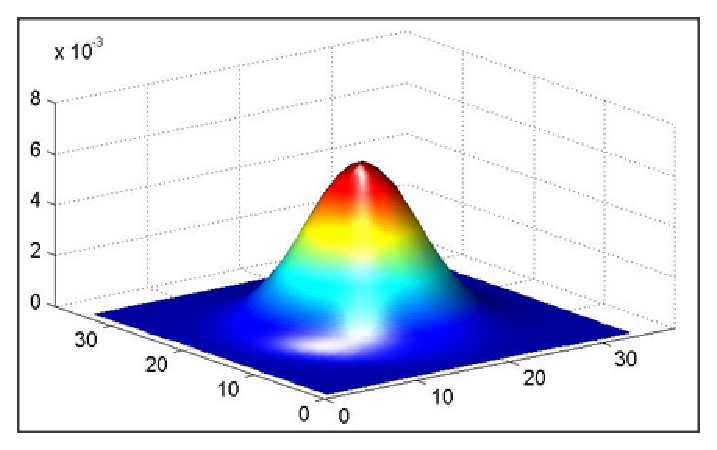
\includegraphics[height=5cm,angle=0]{./images/psf_gaussian.eps}}
  \caption{A sample Gaussian PSF plotted in 3D}
  \label{fig:gaussian_psf}
\end{figure}  

\burl{http://idlastro.gsfc.nasa.gov/ftp/pro/image/psf_gaussian.pro} has
Gaussian PSF function:
\begin{verbatim}
function psf_gaussian, parameters, NPIXEL=npixel, $
                      NDIMENSION=ndim, FWHM=fwhm, $ 
                      DOUBLE = double, CENTROID=cntrd, $
                      ST_DEV=st_dev,  $
                      XY_CORREL=xy_corr, NORMALIZE=normalize
\end{verbatim}


IDL 8.1. has the following new functions
\begin{enumerate}
  \item Smoothing: \verb!GAUSS_SMOOTH! function smoothes data using a Gaussian
  kernel. Also known as a Gaussian blur, it is typically used to reduce noise
  and detail in an image. \verb!EDGE_MIRROR! keyword for CONVOL and SMOOTH and
  the new \verb!EDGE_WRAP! keyword for SMOOTH apply the smoothing function to
  all points. If the neighborhood around a point includes a point outside the array,
  a "mirrored" or "wrapped" edge point is used to compute the smoothed result.  
  \item Convolution: \verb!GAUSSIAN_FUNCTION! function creates a Gaussian kernel
  used in convolution; and \verb!CONVOL_FFT! function computes the convolution
  of an image using a product of Fourier transforms for speed.
\end{enumerate}

  \begin{verbatim}
  psfsigma = 2; % um - point spread function width for optical blurring 
  psf = gaussian(rconv,psfsigma);
  \end{verbatim}

\section{Non-uniform distribution of NCX and SERCA}

\begin{verbatim}
!!setup distribution of SERCA and NCX                                                                                                                                                                                                                                                                                      
CALL tscell_setup_SERCA_NCX()
\end{verbatim}

\section{trigger\_rogue\_RYR}
\label{sec:trigger_rogue_RYR}


\verb!trigger_rogue_RYR! triggers the RYR from the rogue-cluster or the
non-junctional RYR clusters or satellite RYR clusters.

\subsection{trigger\_rogue\_RYR\_3}
\label{sec:trigger_rogue_RYR_3}

\begin{verbatim}
SUBROUTINE trigger_rogue_RYR_3(U_Ro_rogue, CRU_states, NSFU, 
        num_rogueRYRcluster, N_R_rogue, is_all_rogueRYR_open)     
\end{verbatim}


\subsection{trigger\_rogue\_RYR\_4}
\label{sec:trigger_rogue_RYR_4}

This version: designed for macrospark3 simulation where we have 3 rogue clusters
not at the same z-plane in between 2 main CRUs and we trigger the one in the
center
\begin{verbatim}
 SUBROUTINE trigger_rogue_RYR_4(U_Ro_rogue, CRU_states, NSFU, 
num_rogueRYRcluster, N_R_rogue, is_all_rogueRYR_open)     
\end{verbatim}